\section{Introduction}
This project is about the development of the back-end of the bootstrap compiler for the Meta-Casanova 3 language.
The back-end is responsible for generating an executable after receiving the type-checked information from the front-end.

Compilers are complex programs that have to operate on a wide range of inputs.
Since compilers have such a large input-space, the chance of a bug hiding somewhere is substantial. 
But for al their complexity, compilers also have to be bug-free since every program can only be as bug-free as its compiler.

Abstractions can help in this regard.
The limits of which were observed when implementing the compiler for the Casanova language in F\#.
The compiler was 0000 lines long, and became unmaintainable.
After a rewrite in MC it was 000 lines[Maggiore].

EXAMPLE HERE (compare with slow language)

The primary reason for this was the lack of higher-order type operators.
This made abstractions such as monad-transformers impossible, hampering modularity and resulted in a lot of boilerplate code.

In this document, we will walk through the backend and examine the various parts and their design decisions.
In this way, this document aims to be useful to the future developers of the MC compiler.

\subsection{Research questions}

The main research question is: ``What is the best way to implement a backend''  was to develop a backend so typechecked Meta-Casanova(MC) could be transformed into executable code.
In order to do this, several sub-goals were set.

TODO: Convert to questions.

What is the best way to implement the backend?

\begin{enumerate}
    \item decide on the output language.
    \item design a front-end interface and an intermediate representation(IR).
    \item Implement a program to validate the front-end interface and IR.
    \item Implement a Code generator with code mangler.
    \item Implement an interpreter to validate the code generator.
    \item Implement an embedded debugger to help debug the compiler.
\end{enumerate}

To illustrate how the goals relate to each other, here is a diagram of the dataflow through the backend.

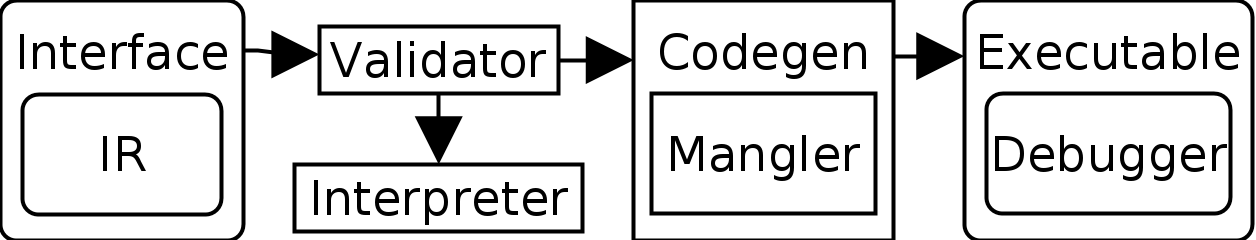
\includegraphics[width=\columnwidth]{overview}

As you can see, the front-end interface contains the IR and goes through the validator.
From there, depending on the compiler flags, it either goes to the interpreter or the codegen.
In case it goes to the interpreter, the program is directly executed.
In case it goed to the codegen, it is translated to the output language.
To translate all the identifiers, the mangler is needed.
The debugger is optionally embedded in the executable, depending on compiler flags.

The sections 3 through 9 go into more detail regarding these subgoals.

\subsection{Requirements}

The project had 3 requiremens.
\begin{enumerate}
    \item The backend must in no case produce an incorrect program.
    \item The executable must be able to inter-operate with .NET.
    \item The generated code must run on all the platforms .NET runs on.
\end{enumerate}
An additional soft requirement was that faster was better.

The first requirement  because the compiler must be reliable.
Any program can at most be as reliable as the compiler used to generate it.

\label{whydotnet}
The second requirement existed because of the need for a large library and inter-operability with Unity game engine.
This is because the main area of research of the organization is game-related.


\subsection{Organization}
--- todo: describe organization ---

